\documentclass[tikz]{standalone}
\usepackage{amsmath}
\definecolor{bg}{HTML}{171D2B}
\definecolor{acc}{HTML}{F7B538}
\definecolor{tx}{HTML}{F8FAFC}
\definecolor{ax}{HTML}{64748B}
\begin{document}
\pagecolor{bg}
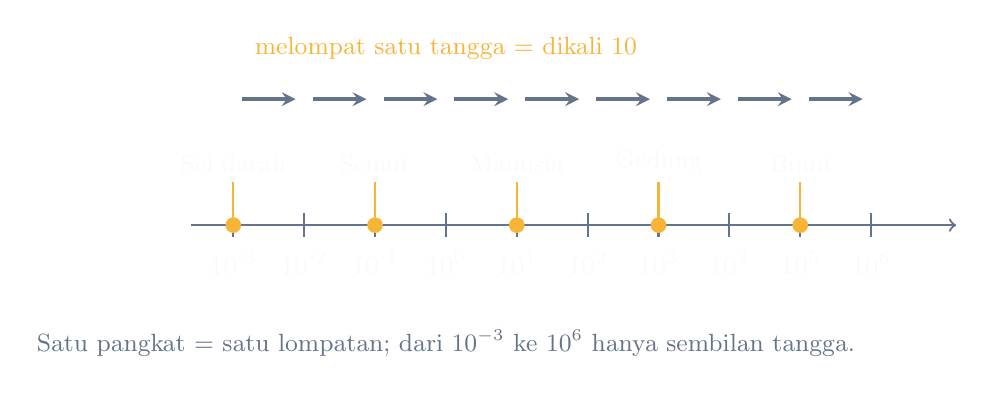
\begin{tikzpicture}[x=0.9cm, y=1cm, text=tx]
  % main axis
  \draw[ax, thick, ->] (-3.6,0) -- (7.2,0);
  \foreach \i/\lab in {-3/{10\textsuperscript{-3}},-2/{10\textsuperscript{-2}},-1/{10\textsuperscript{-1}},0/{10\textsuperscript{0}},1/{10\textsuperscript{1}},2/{10\textsuperscript{2}},3/{10\textsuperscript{3}},4/{10\textsuperscript{4}},5/{10\textsuperscript{5}},6/{10\textsuperscript{6}}}{
    \draw[ax, thick] (\i,-0.15) -- (\i,0.15);
    \node[below=6pt, text=tx] at (\i,0) {\lab};
  }
  % scale markers above
  \foreach \i/\obj/\col in {-3/{Sel darah},-1/{Semut},1/{Manusia},3/{Gedung},5/{Bumi}}{
    \node[circle, fill=acc, inner sep=2pt] (m\i) at (\i,0) {};
    \draw[acc, thick] (\i,0) -- (\i,0.55);
    \node[above, text=tx, font=\small] at (\i,0.55) {\obj};
  }
  % ladder arrows between consecutive powers
  \foreach \i in {-3,...,5}{
    \draw[ax, very thick, ->, >=stealth] (\i+0.12,1.6) -- (\i+0.88,1.6);
  }
  \node[text=acc, font=\small] at (0,2.25) {melompat satu tangga = dikali $10$};
  \node[text=ax, font=\small] at (0,-1.5) {Satu pangkat = satu lompatan; dari $10^{-3}$ ke $10^{6}$ hanya sembilan tangga.};
\end{tikzpicture}
\end{document}
